\chapter[Introdução]{Introdução}
\addcontentsline{toc}{chapter}{Introdução}
\label{chap:introducao}

Neste capítulo, é apresentada uma breve \hyperref[sec:contextualizacao]{Contextualização}, no intuito de deixar mais claro sobre o domínio no qual o trabalho está inserido, bem como para apresentar o problema a ser tratado no mesmo. Neste sentido, é acordada uma definição para privacidade de dados, uma vez que se pretende contribuir para um acompanhamento mais adequado desse topico durante o desenvolvimento do sistema. 

Sendo assim, os domínios de interesse são Aprendizado federado e Privacidade de dados. Pretende-se desenvolver um modelo de treinamento de aprendizado federado e outro modelo com treinamento centralizado a fim de comparar métricas obtidas ao final de cada treinamento. Na sequência, têm-se a \hyperref[sec:justificativa]{Justificativa} para a realização do trabalho e os \hyperref[sec:objetivos]{Objetivos} a serem atingidos. Por fim, há uma breve noção quanto aos \hyperref[sec:metodologia]{materiais e métodos} adotadas no trabalho, e a apresentação da \hyperref[sec:organizacao]{Organização da Monografia}.

\section{Contextualização}
\label{sec:contextualizacao}

A Inteligência Artificial (IA) tem se tornado uma presença cada vez mais marcante em nossas vidas, permeando desde assistentes virtuais até sistemas de recomendação personalizados e sua utilização na indústria, como pode ser visto nos índices de investimentos corporativos globais relacionados a IA (Figura \ref{fig:investimentoIA}).

\begin{figure}[h]
    \centering
    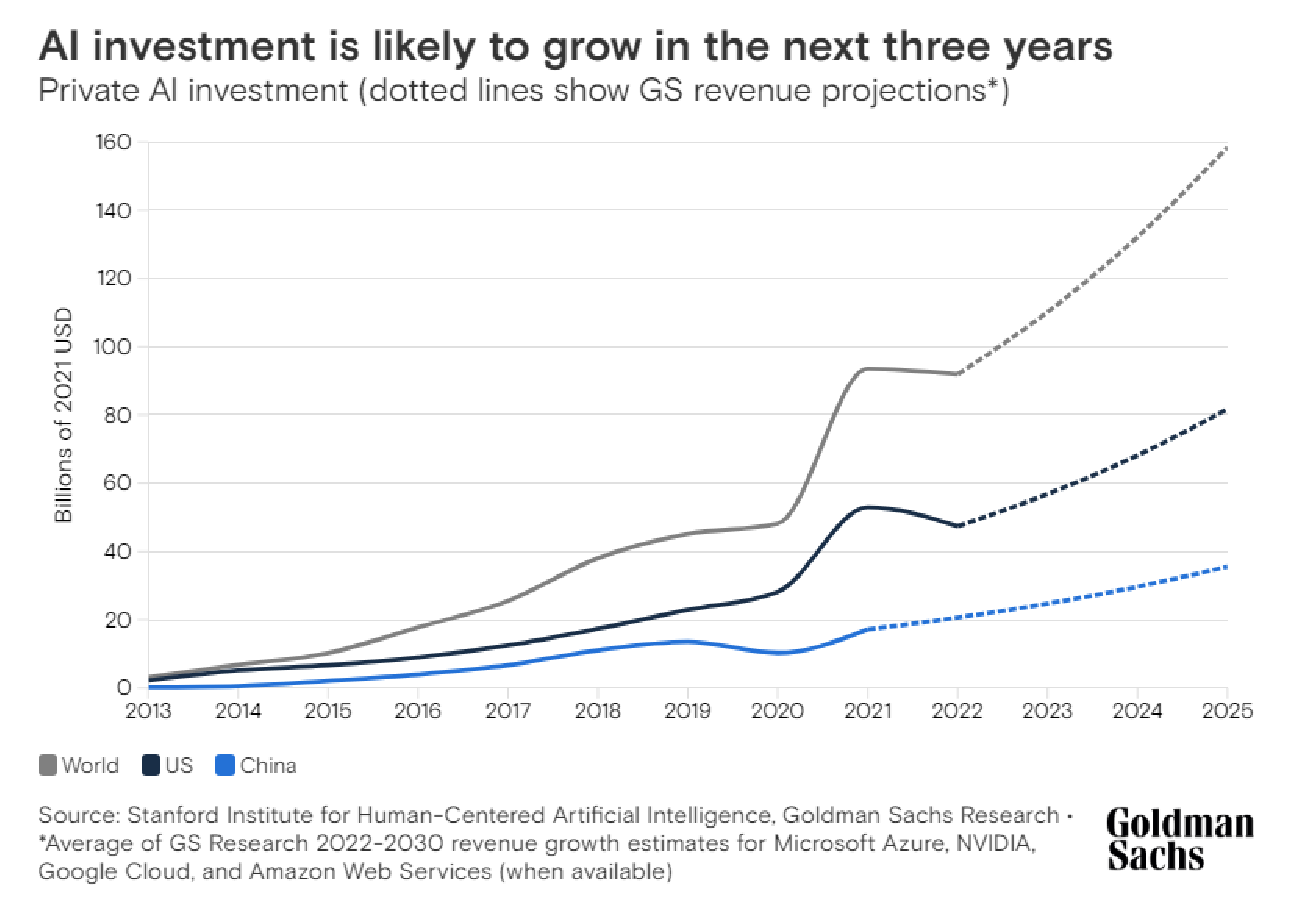
\includegraphics[scale=0.6]{figuras/introducao/AIInvestiments2025.eps}
    \caption{Investimento em IA no setor privado.}
    \label{fig:investimentoIA}
\end{figure}

Essa crescente utilização desses modelos reflete a busca incessante por soluções que otimizem processos, tomem decisões e aprimorem a experiência do usuário, como é refletido nas expectativas sobre o impacto da adoção de modelos de inteligência artificial no mercado de trabalho para os próximos anos, Figura \ref{fig:capacidadeIA}. No entanto, essa onipresença da IA também traz consigo desafios, especialmente quando se trata do tratamento de dados sensíveis e da privacidade dos usuários.

\begin{figure}[h]
    \centering
    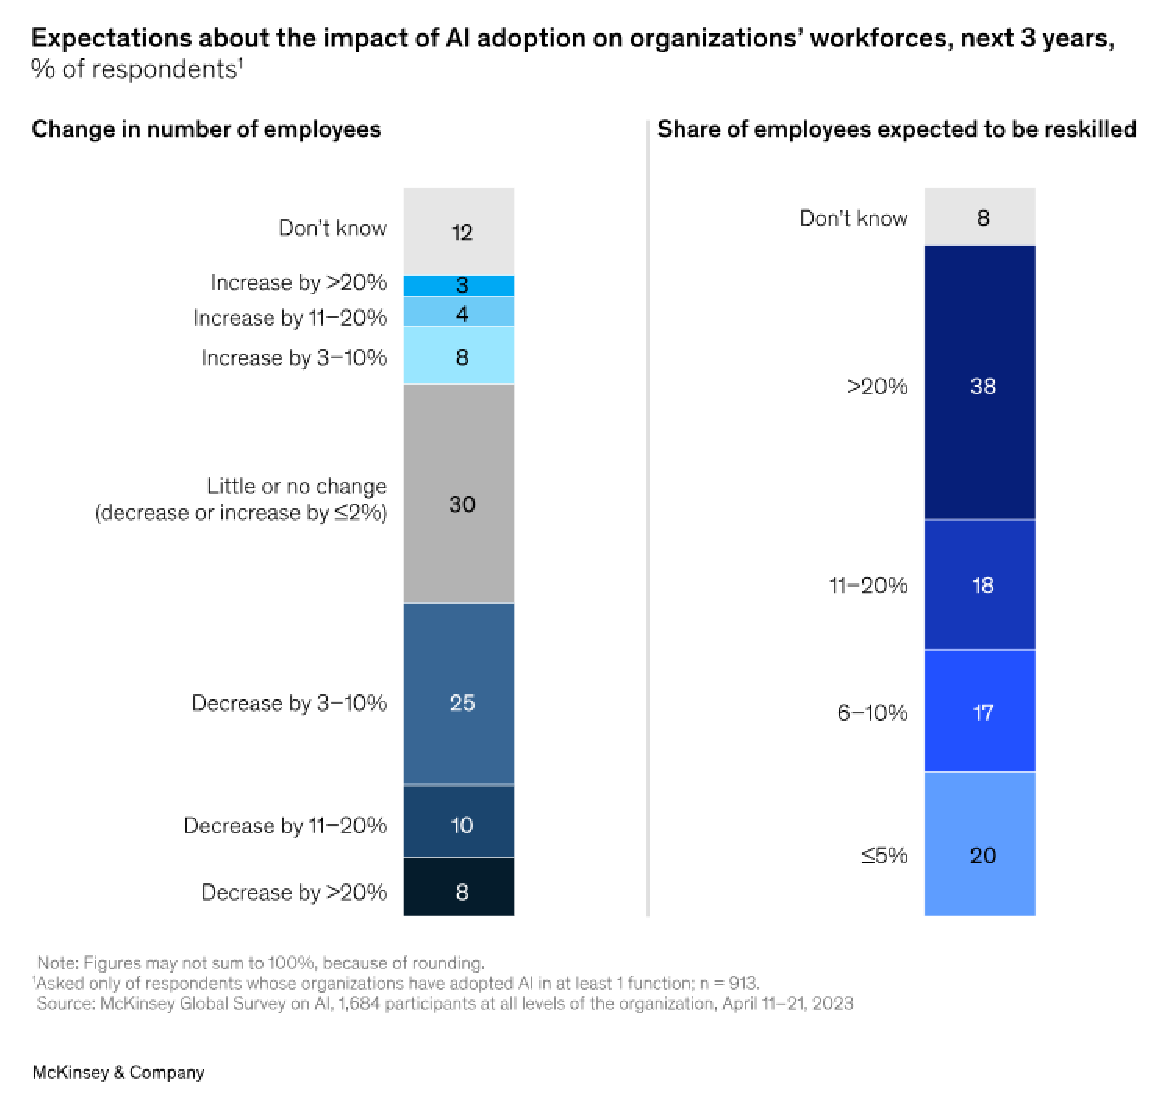
\includegraphics[scale = 0.8]{figuras/introducao/ExpectationsAboutImpact.eps}
    \caption{Expectativas sobre o impacto da adoção de IA's.}
    \label{fig:capacidadeIA}
\end{figure}

A IA, em sua essência, de acordo com a definição mais recente de Stuart Russell, é descrita como o estudo de agentes inteligentes que podem perceber seu ambiente e tomar decisões para alcançar objetivos de forma autônoma. Estes agentes operam em contextos dinâmicos e incertos, ajustando-se ao ambiente para otimizar suas ações. A IA busca construir sistemas que possam agir de maneira racional, onde a "racionalidade" é definida pela capacidade de tomar decisões corretas, maximizando o sucesso com base nas informações disponíveis \cite{russell2022}. No entanto, quando lidamos com dados descentralizados, como os provenientes de dispositivos pessoais, surge um dilema: como treinar modelos eficazes sem comprometer a privacidade dos usuários?

O termo "privacidade de dados" ganhou destaque no campo de tecnologias em resposta à crescente preocupação sobre como as informações pessoais dos indivíduos são coletadas, armazenadas, processadas e compartilhadas. Historicamente, o conceito de privacidade sempre esteve presente, mas a explosão no volume de dados digitais, especialmente com o advento da internet e das redes sociais, trouxe à tona desafios em relação à segurança e à confidencialidade das informações pessoais.

O marco regulatório, como a Diretiva de Proteção de Dados Pessoais da União Europeia (GDPR) \cite{GDPR}, promulgada em 2016, evidencia a crescente importância atribuída à privacidade de dados em nível global. A GDPR estabeleceu normas rigorosas para a coleta e o processamento de dados pessoais, visando proporcionar aos indivíduos um maior controle sobre suas informações pessoais.

O conceito de privacidade no treinamento de redes neurais é amplamente explorado em pesquisas que buscam conciliar a necessidade de dados para treinamento eficaz com a preservação da confidencialidade. Métodos como a privacidade diferencial, proposta por Cynthia Dwork em seu trabalho \textit{"Calibrating Noise to Sensitivity in Private Data Analysis"}\cite{dwork2006calibrating}, introduzem ruído controlado nos dados, garantindo que as contribuições individuais não possam ser identificadas, protegendo assim a privacidade dos participantes no treinamento colaborativo.

Além disso, o aprendizado federado, proposto por McMahan\cite{mcmahan2017communication}, é uma abordagem que permite o treinamento de modelos em dados distribuídos, mantendo os dados localmente nos dispositivos dos usuários.

O aprendizado federado, do inglês federated learning (FL) foi primeiramente descrito por Brendan McMahan como o trecho de tradução própria:

\begin{citacao}
"Nós nomeamos nossa abordagem como Federated Learning, uma vez que a tarefa de aprendizagem é resolvida por uma ampla federação de dispositivos participantes (que chamamos de clientes) que são coordenados por um servidor central \cite{mcmahan2017communication}."
\end{citacao}

Aprendizado de Máquina (AM), conforme descrito por \cite{russell2022} e \cite{goodfellow2016}, refere-se ao campo da inteligência artificial que estuda algoritmos capazes de aprender padrões e tomar decisões com base em dados. A ideia central é que, ao invés de serem explicitamente programados para realizar uma tarefa, os modelos de AM ajustam seus parâmetros com base em grandes conjuntos de dados, de modo a gerar previsões ou classificar informações de maneira autônoma. O objetivo é permitir que as máquinas melhorem seu desempenho à medida que recebem mais informações e exemplos.

A proposta do aprendizado federado no campo de \emph{Machine Learning} (ML) tem suas raízes em questões de privacidade de dados e descentralização. O conceito começou a ganhar destaque no final da década de 2010 como uma abordagem para treinar modelos de ML em dados distribuídos, sem a necessidade de centralizar todos os dados em um único local. Resumindo, FL é um paradigma de aprendizado onde modelos estatísticos são treinados em um sistema distribuído \cite{li2020preserving}.

Em aplicações de FL no mundo real, as partes individuais necessitam de motivação para utilizarem um  sistema de aprendizado federado (FLS), essa motivação pode vir de regulamentações ou incentivos. Quem decide utilizar o FL pode se beneficar com seu modelo de alta precisão\cite{LI}. Por exemplo, hospitais durante a pandemia utilizaram um sistema de ML , treinado utilizando o aprendizado federado, para classificar imagens de torax diferentes fontes (raio-x e ultrassom) com o intuíto de auxiliar no diagnóstico de COVID-19\cite{qayyum2022collaborative}.

Treinar modelos em redes heterogêneas e de grande escala trazem consigo uma nova gama de desafios que requerem uma abordagem fundamentalmente diferente das abordagens tradicionais de treinamento para aprendizado de máquina em larga escala \cite{li3}. Abordaremos durante o capítulo de fundamentação teórica os principais desafios que esse novo paradigma traz consigo, seus benefícios e o que está sendo estudado da área atualmente.

\section{Justificativa}
\label{sec:justificativa}

A necessidade de treinar modelos de inteligência artificial sem comprometer a privacidade dos usuários tem impulsionado a pesquisa em direção ao paradigma do aprendizado federado. A dependência da representatividade dos dados locais, a possível exposição de informações sensíveis durante as atualizações do modelo e a necessidade de garantir a segurança contra ataques são aspectos cruciais a serem abordados.

A diversidade nos conjuntos de dados entre os dispositivos participantes pode levar a modelos globais que não capturam adequadamente as nuances específicas de cada local. A representatividade dos dados locais é discutida em estudos como \cite{mcmahan2017communication}, que ressaltam a importância de estratégias eficientes de agregação para preservar a qualidade do modelo global.

A preservação da privacidade durante o treinamento federado é um ponto crítico, considerando a sensibilidade dos dados envolvidos. Técnicas como privacidade diferencial, discutidas em \cite{shokri2015privacy}, são exploradas para mitigar o risco de divulgação de informações pessoais durante a colaboração no treinamento. No entanto, a aplicação bem-sucedida dessas técnicas requer uma análise cuidadosa das configurações e parâmetros para equilibrar a privacidade e a utilidade do modelo resultante.

A proteção contra ataques que buscam extrair informações dos modelos treinados, é outra dimensão crítica para garantir a segurança. Estudos como "Deep Models Under the GAN: Information Leakage from Collaborative Deep Learning"\cite{hitaj2017deep} destacam a necessidade de estratégias defensivas robustas para preservar a privacidade contra tentativas maliciosas.

A crescente integração de inteligência artificial em nosso cotidiano, especialmente em setores como saúde, finanças e tecnologia, levanta sérias preocupações sobre a privacidade dos dados dos usuários. Incidentes recentes demonstram como a centralização de dados pode resultar em vulnerabilidades significativas. Por exemplo, em 2018, a revelação de que dados de localização de militares dos EUA foram expostos publicamente através de aplicativos de fitness gerou preocupações sobre a segurança nacional \cite{bbc2018strava}. 

Além disso, a coleta indiscriminada de dados por assistentes virtuais, como o caso da Amazon Alexa, trouxe à tona a possibilidade de acesso não autorizado e uso indevido dessas informações pessoais \cite{bloomberg2019amazon}. Escândalos envolvendo redes sociais, como o Facebook e a Cambridge Analytica, ressaltam como a centralização de dados pode ser explorada para influenciar eventos políticos e comprometer a privacidade individual \cite{guardian2018cambridge}. Instituições financeiras também não estão imunes, como evidenciado pelo caso de violação de dados do Capital One\cite{capitalone2019databreach}. 

Esses episódios enfatizam a necessidade de abordagens inovadoras para proteger a privacidade dos usuários e mitigar riscos associados à concentração de dados. O aprendizado federado surge como uma solução promissora neste cenário, permitindo que modelos de machine learning sejam treinados localmente nos dispositivos dos usuários, evitando a necessidade de transferir dados sensíveis para servidores centrais. Essa abordagem descentralizada não apenas preserva a privacidade dos indivíduos, mas também fortalece a segurança dos sistemas de IA, resguardando contra possíveis explorações maliciosas. 

O campo do aprendizado federado não apenas se apresenta como uma resposta pragmática às vulnerabilidades atuais, mas também sinaliza um caminho crítico para a construção de sistemas de IA éticos e seguros em um mundo cada vez mais interconectado.

\section{Questões de Pesquisa e Desenvolvimento}
\label{sec:questoes}

O presente trabalho é de viés aplicado, demandando atividades de pesquisa e desenvolvimento. Portanto, ao final do trabalho, pretende-se responder os seguintes questionamentos:

\textbf{Questão de Pesquisa:} Como o Aprendizado Federado se destaca como uma solução eficaz para o treinamento de modelos de Inteligência Artificial em ambientes descentralizados, e de que maneira ele preserva a privacidade dos usuários durante esse processo?

Diante de estudos preliminares já realizados até o momento, e dada a relevância que a área de Inteligência Artificial vem ganhando nos últimos anos, surge uma crescente preocupacação a respeito de como são distribuídos os dados para treinamento dos modelos. O objetivo deste estudo é explorar e analisar a aplicabilidade do modelo de treinamento do aprendizado federado para a preservação e manutenção da privacidade de dados dos usuários. Demais informações sobre o tema serão apresentadas no \hyperref[chap:teorico]{Capítulo 2 - Referencial Teórico}.

\textbf{Questão de Desenvolvimento:} Quais são os desafios e limitações associados à implementação prática do AF em cenários descentralizados, especialmente em termos de eficiência computacional, comunicação entre dispositivos e adaptação a diferentes tipos de dados?

A implementação prática do Aprendizado Federado em cenários descentralizados enfrenta desafios que afetam sua eficiência computacional, a comunicação entre dispositivos e a adaptação a diferentes tipos de dados. Primeiramente, a heterogeneidade de dispositivos e redes pode resultar em variações significativas na eficiência do treinamento. A comunicação entre dispositivos é limitada por questões de largura de banda e latência, impactando diretamente a sincronização eficiente dos modelos federados. Adicionalmente, a diversidade nos tipos de dados distribuídos impõe desafios na harmonização e adaptação de modelos para garantir a generalização adequada.

Neste sentido, há uma necessidade de um estudo mais criterioso sobre como desenvolver um modelo que atenda a estas preocupações. O desenvolvimento busca acompanhar e compreender como o AF pode atuar como uma solução para o treinamento descentralizado de modelos de inteligência artificial, realizando de maneira efetiva o processamento dos dados e mantendo a privacidade dos usuários.

\section{Objetivos}
\label{sec:objetivos}

A proposta desse trabalho visa explorar e analisar a aplicabilidade do Aprendizado Federado no contexto do treinamento de modelos de Inteligência Artificial em ambientes descentralizados. Este estudo é motivado pela crescente importância de preservar a privacidade dos usuários em um cenário em que dados sensíveis estão distribuídos em dispositivos diversos, como dispositivos móveis, sensores IoT e servidores locais.

O diferencial desta pesquisa reside na abordagem abrangente e aprofundada do AF em ambientes descentralizados, focando não apenas nos aspectos técnicos, mas também nas implicações éticas e práticas associadas. Ao considerar a heterogeneidade de dados, desafios de comunicação, e a necessidade crítica de proteger informações sensíveis, este estudo visa oferecer insights valiosos para o desenvolvimento e implementação eficaz de sistemas de IA federados.

A importância deste trabalho é evidenciada pela urgência de encontrar soluções que conciliem os avanços em IA com a proteção da privacidade individual. À medida que a coleta e o processamento de dados descentralizados se tornam a norma, a comunidade científica e a indústria enfrentam o desafio de assegurar que os modelos de IA derivados desses dados não comprometam a privacidade dos usuários. Neste contexto, o AF surge como uma abordagem promissora, e este trabalho busca contribuir para a compreensão profunda de suas implicações, desafios e melhores práticas.

As contribuições deste estudo para a área de IA são diversas. Primeiramente, espera-se fornecer diretrizes práticas para a implementação bem-sucedida do AF em ambientes descentralizados, considerando os aspectos práticos e éticos. Além disso, ao abordar questões de segurança e conformidade com regulamentações de privacidade, este trabalho busca fortalecer a confiança na aplicação do AF. Por fim, ao delinear as possíveis evoluções futuras do AF e seu papel na preservação da privacidade, este estudo visa inspirar pesquisas subsequentes e avanços na área.

Neste contexto, o \textbf{Objetivo geral} é investigar como o treinamento de inteligências artificiais por meio do aprendizado federado pode ser efetivamente aplicado no contexto de dados descentralizados. 

Com o norte do objetivo geral e sua abrangência prevista, pretende-se atingi-lo através do cumprimimento de alguns \textbf{Objetivos específicos} sendo eles: 

\begin{itemize}
    \item Objetivo específico 1: Conceituar Aprendizado federado e apontar as estratégias de aprendizado de máquina que podem ser usadas para preservação da privacidade dos usuários e de dados sensíveis.
    \item Objetivo específico 2: Discorrer sobre técnicas de segurança e privacidade necessárias para proteger os dados dos usuários e o provedor do serviço durante o processo de treinamento.
    \item Objetivo específico 3: Analisar o problema de uso de dados decentralizados, identificando os principais desafios.
    \item Objetivo específico 4: Comparar a eficácia do modelo de treinamento descentralizado quando comparado com modelos tradicionais de treinamento.
\end{itemize}

É importante salientar que, para cumprimento desses objetivos, sobre a necessidade de orientação por metodologias de:
\begin{itemize}
    \item pesquisa, para condução dos estudos e levantamentos;
    \item desenvolvimento, para construção da solução em si, e
    \item análise de resultados, para lidar mais adequadamente com os resultados obtidos.
\end{itemize}
.

\section{Materiais e Métodos}
\label{sec:metodologia}

No capítulo de materiais e métodos, serão tratados os aspectos metodológicos do trabalho de forma mais adequada. Entretanto, visando esclarecer alguns pontos, o trabalho pode ser classificado segundo \cite{GIL}, quanto:

\begin{itemize}
    \item \textbf{Quanto aos objetivos}: a pesquisa é classificada como exploratória, pois busca explorar o tema do aprendizado federado e sua aplicabilidade no treinamento de modelos de IA em ambientes descentralizados, bem como investigar os desafios e limitações associados à implementação prática do AF.
    \item \textbf{Quanto aos procedimentos técnicos}: a pesquisa é classificada como bibliográfica-experimental, pois envolve a revisão de literatura sobre aprendizado federado, privacidade de dados, segurança em IA e tópicos relacionados assim como o desenvolvimento de modelos que servirão como objetos de estudo para definição de formas de controle e observação dos efeitos que a variável produz no objeto.
    \item \textbf{Quanto à abordagem do problema}: a pesquisa é classificada como Quali-quantitativas, pois busca compreender e analisar os aspectos práticos e éticos do AF em ambientes descentralizados, considerando a heterogeneidade de dados, desafios de comunicação e a necessidade de proteger informações sensíveism, combinando a análise de métricas e números gerados com os experimentos.
\end{itemize}

\section{Organização}
\label{sec:organizacao}

A monografia está organizada em capítulos, conforme a seguir:

\begin{itemize}
    \item Capítulo 1 - Fundamentação Teorica: Neste capítulo, são apresentados os conceitos fundamentais relacionados ao aprendizado federado, privacidade de dados, segurança em IA e tópicos relacionados. O objetivo é fornecer uma base teórica sólida para a compreensão do tema e a análise dos resultados.
    \item Capítulo 2 - Referencial Tecnológico: descreve as principais tecnologias, ferramentas e frameworks, ou seja, o arcabouço tecnológico que viabilizou não apenas o desenvolvimento da solução em si, mas também seu planejamento, sua especificação e sua análise;
    \item Capítulo 3 - Materiais e métodos: descreve os procedimentos técnicos e metodológicos adotados para a realização do trabalho, incluindo a revisão bibliográfica, a coleta de dados, a análise dos resultados e a avaliação da solução proposta;
    \item Capítulo 4 - Desenvolvimento: descreve o desenvolvimento da solução proposta, a implementação dos modelos de IA, a integração com as tecnologias selecionadas e os resultados obtidos;
    \item Capítulo 5 - Análise de Resultados: apresenta a análise dos resultados obtidos, a comparação entre os modelos de IA treinados e a discussão sobre os desafios e limitações identificados;
    \item Capítulo 6 - Conclusão: apresenta as conclusões finais do trabalho, destacando as contribuições, as limitações e as sugestões para trabalhos futuros.
\end{itemize}